\chapter{Chapter Title}

This chapter contains examples of LaTeX code in action.
To look at and work with the underlying templates, switch to the corresponding position in the .tex file by hitting "Ctrl + LeftClick" here, i.e. inside the Pdf Viewer of Texmaker.

\section{Section Title}

Chapters are divided into sections.

\subsection{Subsection Title}
\label{text:subsection}
Sections are further divided into subsections.

\subsubsection{Subsubsection Title}
For even finer subdivision of text you can add another sub-prefix.

\paragraph{Paragraph Title}

A paragraph is the lowest level of text subdivision. 
Note that the paragraph title is put in line with the bulk text.

\section{Automatic Numbering}

For any new definition, LaTeX creates an automatic numbering.
This applies to text structures like chapters, sections and paragraphs, as well as to additional environments like tables, figures and equations.
Examples can be found in table \ref{tab:keyboard-shorts}, figure \ref{fig:xkcd} and equation ??.

By default, the text numbering is active down to subsection level, as shown in subsection \ref{text:subsection} above.

By the way: Did you notice how the mouse pointer changes to a hand symbol when hovering over the subsection number above?
Whenever the hand symbol is visible, you are pointing onto a dynamic link, which can be used to jump to the corresponding label.

\subsection{Extend Numbering to Lower Levels}

If additional sub-levels need to be numbered, include one of the two following code snippets into the header file "packages.tex".

To number down to subsubsections but leave paragraphs without number:
\lstinputlisting{files/chapters/chapter-1-sections/extend-numbering-lvl3-subsubsections.tex}

To number paragraphs as well:
\lstinputlisting{files/chapters/chapter-1-sections/extend-numbering-lvl4-paragraphs.tex}


\section{Label for a Reference}

To refer to a specific position inside a LaTeX report, declare a label.
\label{text:a-label-position}
This label is only visible in the LaTeX editor and not printed into the final pdf. To find the hidden label in this section, hit "Alt+LeftClick" right here inside the "Pdf Viewer".

Labels can be placed in special environments like tables, figures and equations as well.

\section{Reference to a Label}

As seen in section \ref{text:a-label-position}, a reference needs a label to work.
Inside the pdf generated by LaTeX, you can click on any reference to jump to the corresponding label position.
This possibility is visualized by the mouse pointer changing to a hand symbol with one finger pointing upward.

\hyperlink{toc:label}{It's also possible to customize links, e.g. to jump to the table of contents.}

\subsection{Jump Back to Label Position}

After following a link inside the output pdf, you can press "Alt+LeftArrow" to jump back to the original position inside the pdf.
For this feature to work, the pdf has to be opened outside the Texmaker program, e.g. with the \url{https://get.adobe.com/reader/}.


\section{Commenting}

To write a comment in your .tex file, start a new line with "\%".
Commented code parts are ignored by the compiler.


\section{Include .tex Files}
\label{text:include-files}




\section{Figure}

\subsection{Single Image}

% {figure}[H] or {figure}[htb]
% [H] enforces the figure to be exactly here
% [htb] allows the figure to be placed either here, on top or at the bottom of the page. Checking for suitable location in this order (first h, 2nd t, last b).

\begin{figure}[H]
  \begin{center}
    % \includegraphics[attr1=val1, attr2=val2, ...]{imagepath/imagename}
    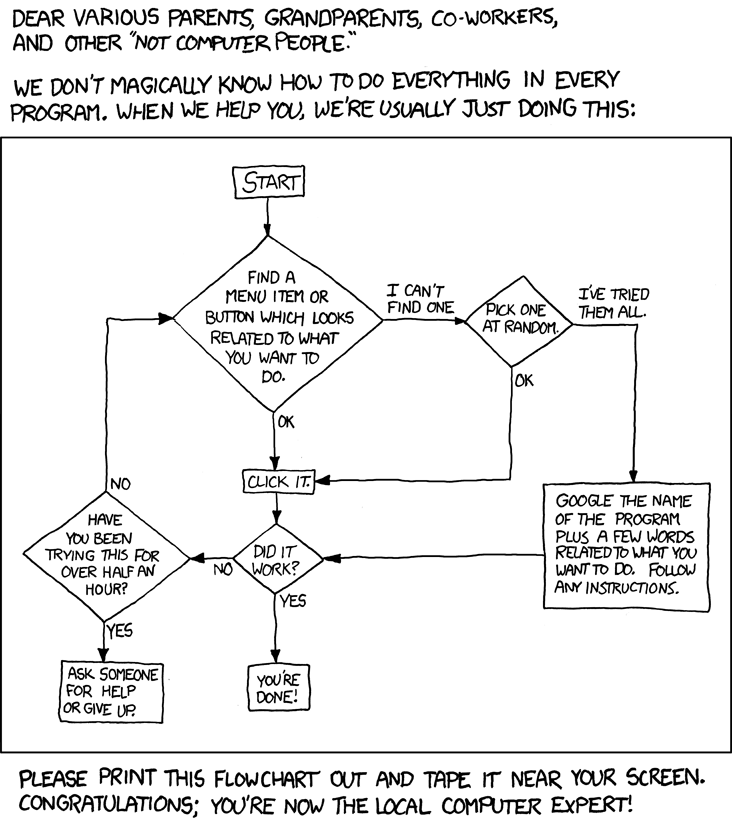
\includegraphics[width=0.75\columnwidth]{files/images/xkcd_tech_support_cheat_sheet.png}
  \end{center}
  \caption{On how to become a local computer expert. \\ Don't forget "Ctrl+LeftClick" here :) }
  % \\ = new line
  % call caption before label
  \label{fig:xkcd}
\end{figure}


\subsection{Multiple Images}




\section{Citation}

To cite bibliography sources in LaTeX, I recommend using JabRef. 
JabRef is an open source graphical application for managing bibliographical data.

Besides standard citations like books \cite{2000_Kuffel_HV_engineering_fundamentals} or articles \cite{2004_Whitesides_writing_a_paper}, JabRef can also be used to define custom entry types like webpages for example \cite{2015_github_webpage}.


\section{Nomenclature Entries}

Technical terms and abbreviations used inside a report can be gathered using a nomenclature (see section \ref{text:nomenclature}).

Define new nomenclature entry, e.g. a specific abbreviation, inside the separate file nomenclature.tex 

ref ??.
This definition can then be linked to usages of the technical term inside the report.
%\phantomsection \label{def:tg}
%Thermogravimetric measurements are performed with a \acs{tg}.

%\subsection{subsection name}
%
%To address the diffusion limitations encountered by \acs{tg}, a packed bed tubular reactor (\phantomsection \label{def:pb} \acs{pb}) has been developed. \lipsum[2] 


\section{Switch to German Output Language}

Switch language-specific output to German by calling:

\lstinputlisting{files/chapters/chapter-1-sections/switch-language-to-german.tex}

 as the first package in the header file "packages.tex".
As an example, "Contents" then becomes "Inhaltsverzeichnis" and "Bibliography" becomes "Quellenverzeichnis".


\section{Filler Text}

Here's an example of filler text, e.g. to test the appearance of a new font setting.

\lipsum[1]

\section*{Suppress Numbering}
\addcontentsline{toc}{section}{Suppress Numbering}

To suppress numbering of a particular LaTeX object add "*" between object call and curly brackets.
As an example, the current section was created by:

\lstinputlisting{files/chapters/chapter-1-sections/suppress-numbering.tex}

This can be useful to separate certain parts like the nomenclature or appendix from the main text.
Suppressing the numbering also prevents enumeration in the table of contents. 
To still create an entry in the \hyperlink{toc:label}{table of contents}, call the following code just after creating the suppressed section:

\lstinputlisting{files/chapters/chapter-1-sections/suppress-numbering-into-toc.tex}
